%%
%
% ARQUIVO: main.tex
%
% VERSÃO: 1.1
% DATA: Janeiro de 2016
% AUTOR: Coordenação PPgSC
% 
%  Arquivo tex principal do documento de Dissertação.
%  Este arquivo SÓ PRECISA SER MODIFICADO NA PARTE DE CONTEÚDO:
%
%    a. colocar um \include{•} para cada capítulo da Dissertação.
%
%%

% -----
% CLASSE DO DOCUMENTO DA PROPOSTA DE DISSERTAÇÃO
% -----
\documentclass{proposta}

% -----
% PACOTES LATEX USADOS NO DOCUMENTO DA PROPOSTA DE DISSERTAÇÃO
% -----
\usepackage[brazilian]{babel}
\usepackage[utf8]{inputenc}
\usepackage[T1]{fontenc}

\usepackage{amsmath}
\usepackage{graphicx}
\usepackage{tabularx}
\usepackage{float}
\usepackage{color}
\usepackage{amsfonts,amssymb}
\usepackage[authoryear]{natbib}

\usepackage{enumitem}
\usepackage{rotating}
\usepackage{lipsum}
\usepackage{lastpage}
\usepackage{stringstrings}
\usepackage{pgffor}

% -----
% MARGENS DO DOCUMENTO DA PROPOSTA DE DISSERTAÇÃO
% -----
\usepackage{geometry}
\geometry{
	a4paper,
	total={210mm,297mm},
	left=25mm,
	right=25mm,
	top=25mm,
	bottom=30mm,
	textwidth=160mm,
	textheight=242mm,
	headheight=0mm,
	headsep=0mm,
}

% -----
% DECLARAÇÕES AUXILIARES PARA REFERÊNCIAS
%
%  Diferencia \citet e \citep de acordo com a NBR 10520:2002
% -----
\DeclareRobustCommand{\NATand}{;}
\DeclareRobustCommand{\NATetal}{et~al.}
\makeatletter
\renewcommand{\NAT@nmfmt}[1]{%
  \ifNAT@swa\expandafter\MakeUppercase
  \else\DeclareRobustCommand{\NATand}{ e}\expandafter\@firstofone\fi{{\NAT@up #1}}%
}
\makeatother

% -----
% AMBIENTE DE FIGURAS DA PROPOSTA DE DISSERTAÇÃO
%
%  A classe do documento está configurada SOMENTE para figuras no formato EPS.
%  Logo, use PREFERENCIALMENTE este tipo de arquivo.
%
%    a. os arquivos das figuras devem estar no diretório 'img'
% -----
\graphicspath{{./img/}}

% -----
% INÍCIO DO DOCUMENTO DA PROPOSTA DE DISSERTAÇÃO
% -----
\begin{document}

% -----
% DADOS DA PROPOSTA DE DISSERTAÇÃO
%  ALTERAR o arquivo dados-proposta.tex
% -----
%%
%
% ARQUIVO: dados-proposta.tex
%
% VERSÃO: 1.1
% DATA: Janeiro de 2016
% AUTOR: Coordenação PPgSC
% 
%  Arquivo tex com os dados acerca da Proposta de Dissertação.
%
%
%%

%%% AUTOR DA PROPOSTA DE DISSERTAÇÃO (Nome completo)
\autor{Ricardo de Azevedo Brandão}

%%% CÓDIGO DO AUTOR DA PROPOSTA DE DISSERTAÇÃO
\codigoautor{SC 16113}

%%% POSTO DO AUTOR DA PROPOSTA DE DISSERTAÇÃO
% ---
%  se o autor é CIVIL, REMOVA ESTA LINHA
%  se o autor é MILITAR, coloque CORRETAMENTE o POSTO aqui
% ---
%\postoautor{1 Ten}

%%% TITULO DA PROPOSTA DISSERTAÇÃO
\titulo{Mineração de Dados Distribuída Aplicada à Detecção de Desvios Comportamentais no Contexto da Internet das Coisas}

%%% DATA DA APRESENTAÇÃO (formato {dd}{Mmmmm}{aaaa})
\dataapresentacao{13}{dezembro}{2016}

%%% ÁREA DE CONCENTRAÇÃO DA PROPOSTA DISSERTAÇÃO
% ---
%  VER SITE do PPGSC para ver as Áreas de Concentração do Programa.
%  Em 2016 só existe uma Área de Concentração:
%     Ciência da Computação
% ---
\area{Sistemas e Computação}

%%% LINHA DE PESQUISA DA PROPOSTA DISSERTAÇÃO
% ---
%  VER SITE do PPGSC para ver as Linhas de Pesquisa do Programa.
%  Em 2016 só existem três Linhas de Pesquisa:
%     Metodologia da Computação
%     Sistemas de Computação
%     Engenharia de Sistemas e Informação
% ---
\linha{Engenharia de Sistemas e Informação}

%%% ORIENTADOR DA PROPOSTA DE DISSERTAÇÃO
% ---
%  CAMPO 1: Nome completo
%  CAMPO 2: D (para D.Sc.); P (para Ph.D.); ou qualquer coisa (inclusive VAZIO) - o que for escrito aparecerá no documento
% ---
\orientador{Ronaldo Ribeiro Goldschmidt}{D}

%%% POSTO DO ORIENTADOR DA PROPOSTA DE DISSERTAÇÃO
% ---
%  se o orientador é CIVIL, REMOVA ESTA LINHA
%  se o orientador é MILITAR, coloque CORRETAMENTE o POSTO aqui:
%     pode ser: 1 Ten; Cap; Maj; Ten Cel; Cel
% ---
%\postoorientador{Ten Cel}

%%% CO-ORIENTADOR DA PROPOSTA DE DISSERTAÇÃO
% ---
%  se NÃO HOUVER co-orientador, REMOVA ESTA LINHA
%  preenchimento idêntico a \orientador{}{}
% ---
%\coorientador{Nome Completo do Co-orientador}{P}

%%% POSTO DO CO-ORIENTADOR DA PROPOSTA DE DISSERTAÇÃO
% ---
%  se NÃO HOUVER co-orientador, REMOVA ESTA LINHA
%  caso contrário
%    se o co-orientador é CIVIL, REMOVA ESTA LINHA
%    se o co-orientador é MILITAR, coloque CORRETAMENTE o POSTO aqui:
%       pode ser: 1 Ten; Cap; Maj; Ten Cel; Cel
% ---
%\postocoorientador{Cap}

%%% COORDENADOR DE PÓS-GRADUAÇÃO
% ---
%  CAMPO 1: Nome completo
%  CAMPO 2: D (para D.Sc.); P (para Ph.D.); ou qualquer coisa (inclusive VAZIO) - o que for escrito aparecerá no documento
% ---
\coord{Ronaldo Moreira Salles}{P}

%%% POSTO DO COORDENADOR DE PÓS-GRADUAÇÃO
% ---
%  se o Coordenador de PG é CIVIL, REMOVA ESTA LINHA
%  se o Coordenador de PG é MILITAR, coloque CORRETAMENTE o POSTO aqui:
%     pode ser: 1 Ten; Cap; Maj; Ten Cel; Cel
% ---
\postocoord{Cel}

%%% CHEFE DA SEÇÃO (SE/8)
\chefe{Luiz Henrique da Costa Araújo}

%%% POSTO DO CHEFE DA SEÇÃO (SE/8)
% ---
%  se o Chefe é CIVIL, REMOVA ESTA LINHA
%  se o Chefe é MILITAR, coloque CORRETAMENTE o POSTO aqui:
%     pode ser: 1 Ten; Cap; Maj; Ten Cel; Cel
% ---
\postochefe{Cel}



% -----
% PARTE PRÉ-TEXTUAL DA PROPOSTA DE DISSERTAÇÃO
% -----
\makecapa
\maketitle

\parindent 0.75cm


% -----
% PARTE DE CONTEÚDO DE SUA PROPOSTA DE DISSERTAÇÃO
%
% Alterar o conteúdo dos arquivos capitulo-02.tex / capitulo-03.tex / capitulo-04.tex
% -----
% -----
% ARQUIVO: capitulo-02.tex
% VERSÃO: 1.1
% DATA: Janeiro de 2016
%
% CAPÍTULO DE INTRODUÇÃO DA PROPOSTA
%
% NÃO MEXA NAS SEÇÕES, SOMENTE EDITE O CONTEÚDO.
% -----

\chapter{Introdução} \label{chap:Intro}
% #TXT_INTRODUCAO
O avanço tecnológico que possibilitou a redução de tamanho de processadores, aliado ao aumento de capacidade de processamento abriu caminho para uma proliferação de equipamentos integrados com sensores, atuadores, RFIDs (Radio-Frequency IDentification), smartphones e dispositivos sem fio a serem utilizados para os mais diversos propósitos. Havia uma tendência natural que esses dispositivos se conectassem à internet a fim de compartilhar os dados coletados com nós geograficamente dispersos e permitir que usuários pudessem enviar comandos para esses objetos de remotamente.

Ao longo do tempo, mesmo que não tenhamos dado conta, essas "coisas" começaram a fazer parte de nossas vidas alterando significativamente a forma como os indivíduos se relacionam.

%Lembrando que serão utilizados os termos dispositivos, objetos e coisas para representar qualquer equipamento conectado à internet.

Para representar essa extensão da internet que rompeu os limites das redes de computadores, participando de forma pervasiva no dia a dia das pessoas, foi cunhado o termo Internet das Coisas.

De acordo com \cite{000-000} a Internet das coisas nasceu com o propósito ousado de conectar todas as coisas do mundo na internet. O que está causando um grande impacto no dia-a-dia e no comportamento das pessoas, \cite{000-003}, uma vez que está se inserindo em diversas áreas como por exemplo transporte, ambientes domésticos, indústria, logística, saúde e entretenimento. A cada dia um novo sistema ou aplicação é incluído nesse ecossistema, de forma que hoje, a grande maioria de nossas atividades diárias estão sendo controladas ou monitoradas por um dispositivo conectado à internet.

A indústria e a academia têm trabalhado na construções de ambientes compostos por sistemas inteligentes em diversas áreas como casas inteligentes, transporte, logística e saúde \cite{000-000}.

%Outra linha de pesquisa tem aprofundado a questão da arquitetura dos dispositivos como em \cite{000-006} no qual é proposta uma análise abrangente do estado da arte da Internet das coisas abordando uma proposta de desenho de arquitetura de três camadas: (i) Tecnológica, (ii) Acesso (iii) Internet, (iv) \textit{Middleware} e (v) Aplicação. Já em \cite{000-003} o autor aprofunda o assunto com foco no desenvolvimento para dispositos de Internet das Coisas, detalhando os quesitos técnicos da arquitetura.
%
%Porém, uma das mais importantes questões que tem surgido é como converter os dados gerados ou capturados pela Internet das Coisas em conhecimento \cite{000-000}. Então diversas técnicas de KDD (\textit{Knowledge Discovery in Databases}) e Mineração de dados têm sido aplicadas para analisar os dados com o objetivo de melhorar os serviços providos pelos ambientes formados por esses dispositivos.

\section{Contextualização} \label{sec:context}
% #TXT_CONTEXTUALIZACAO

A quantidade de dados geradas pelos dispositivos gera grandes oportunidades de extrair informações valiosas com a utilização de técnicas de KDD (\textit{Knowledge Discovery in Databases}) e Mineração de dados, mas por outro lado traz grandes desafios no gerenciamento dos dados devido ao volume, heterogeneidade, dispersão e questões temporais, dos dados gerados pelas coisas.

De acordo com \cite{000-000} a quantidade de dados gerados em um ano já excede a 1 zetabyes ($10^{21}$ bytes). As ferramentas de análise de dados disponíveis atualmente não são poderosas o suficiente para lidar com uma quantidade tão grande de dados, isso sem contar com as questões de armazenamento e capacidade de transmissão de todo esse volume de informação entre as coisas e os nós centrais de processamento. Curiosamente o gargalo no tratamento dos dados, nesse contexto, aos poucos é transferido dos sensores para o processamento, comunicação e armazenamento.

Os dados na Internet das Coisas podem ser classificados em dados sobre as coisas, como estado, localização, etc e dados gerados pelas coisas. Esses últimos contém dados representativos das interações entre: (i) coisas, (ii) humanos e coisas e (iii) entre humanos \cite{000-018}. 

Assim, ao utilizar técnicas de detecção de padrões é possível identificar o comportamento das coisas e dos humanos cujos dados são coletados pelos dispositivos, que por sua vez possibilitam identificar desvios comportamentais dos objetos e pessoas monitorados. 

\section{Trabalhos Relacionados} \label{sec:trabRelac}

Os trabalhos relacionados foram divididos em três grupos: \begin{itemize}
    \item \textbf{Mineração de Dados na Internet das Coisas}: Apresentam o estado da arte da Mineração de dados na Internet das Coisas. Apresentam os desafios e os problemas abertos.
    \item \textbf{Mineração de Dados Distribuída}: Trabalhos com técnicas de mineração distribuída, não necessariamente no contexto da Internet das Coisas. \linebreak
    Apresentarão bases para análise e projeto dos algoritmos e técnicas que serão desenvolvidos  para o atingimento do objetivo.
    \item \textbf{Detecção de Desvios}: Trabalhos relacionados com identificação de padrões com geração de modelos e detecção de desvios de comportamento no monitoramento de atividades.
    \end{itemize}

\subsection{Mineração de Dados na Internet das Coisas}

\begin{enumerate}

    \item \cite{000-000}: Um Survey abrangente sobre mineração de dados no contexto da Internet das Coisas. Discorre sobre as diversas técnicas de mineração de dados aplicadas ao contexto da Internet das Coisas relacionando-as com seus usos: infraestrutura e serviços. Apresenta os principais problemas abertos, divididos nos seguintes grupos: \begin{itemize}
        \item Infraestrutura
        \item Dados
        \item Algoritmos
        \item Segurança e Privacidade
    \end{itemize}
    Aborda o fato dos principais algoritmos de mineração de dados serem centralizados, o que pode, em pouco tempo inviabilizar suas utilizações em Internet das Coisas devido à sobrecarga causada nas redes de dispositivos na transferência de grande quantidade de dados.

    \item \cite{000-014}: São abordados os desafios na mineração de redes de sensores sem fio -- WSN (\textit{Wireless Sensor Networks}. Tem como foco analisar o trade-off entre: \begin{itemize}
        \item Mineração centralizada com alto consumo de rede para transferência de dados
        \item Mineração nos sensores com limitações: \begin{itemize}
            \item Capacidade de processamento
            \item Consumo de Energia
            \item Tempo de vida das baterias
        \end{itemize}
    \end{itemize}
 
    \item \cite {003-000}: A partir da preocupação com o grande volume de dados, o trabalho propõe quatro diferentes modelos de mineração de dados para Internet das coisas: \begin{itemize}
        \item Modelo multicamada
        \item Modelo de Mineração Distribuída
        \item Mineração de Dados baseada em Grid
        \item Modelo baseado numa perspectiva multitecnológica.
    \end{itemize}

    Após a descrição dos modelos, são apresentados alguns dos problemas abertos e uma discussão sobre a utilização de mineração centralizada versus descentralizada. 
    
\end{enumerate}

\subsection{Mineração de Dados Distribuída}

\begin{enumerate}

    \item \cite{001-000}: Nesse trabalho é apresentado o GDCluster, um algoritmo genérico de clusterização descentralizada. 
    Tem como proposta que cada nó faça uma sumarização de seus dados e compartilhe com seus vizinhos. O resultado final é atingido analisando os dados internos com os dados sumarizados recebidos dos demais nós. Isso é feito de forma iterativa até que se chegue no nó central.
    O algoritmo considera o dinamismo dos dados, atribuindo uma idade a cada item do \textit{dataset}.
    
    % Colocar figura? 
    
    \item \cite{017-000}: Apresenta o $D^{2}CA$ (\textit{Distributed Dynamic Clustering Algorithm}), um algoritmo que explora a clusterização de forma distribuída, maximizando o paralelismo e minimizando a comunicação. Tem como rotina básica: \begin{itemize}
        \item Modelos locais gerados por clusterização K-means
        \item Cálculo dos contornos (usados como representantes dos clusters)
        \item Troca de contornos entre nos vizinhos
        \item Fusão dos contornos em grupos
        \item Escolha de um líder entre os nós
        \item Repetição do processo até atingir o nó central.
    \end{itemize}
    

\end{enumerate}

\subsection{Detecção de Desvios}

\begin{enumerate}
    \item \cite{022-000}: Propõe uma nova formulação na detecção de \textit{outliers} com base na distância, utilizando um algoritmo baseado em partições
    \item \cite{023-000}: Utiliza o algoritmo LOF (\textit{Local Outlier Factor}) aplicado em um grid com o objetivo de reduzir o tempo de computação na descoberta de desvios de comporamento.
\end{enumerate}

\section{Problema} \label{sec:problema}

O grande volume gerado sobre e pelas coisas necessitam de análise de dados não só pelas especificidades de cada aplicação (negócio ou infraestrutura) mas também no sentido de compreender o modo como a Internet das Coisas está se inserindo na vida das pessoas assim como os impactos que causará na sociedade.

Considerando o crescente volume de dados neste cenário, a tradicional reunião dos dados coletados de forma distribuída visando análises centralizadas tende a ser inviável \cite{000-000}.

Aliado ao exposto, muitas aplicações de Internet das Coisas estão voltadas à segurança das pessoas, como os trabalhos apresentados por \cite{000-109}, \cite{000-112}, \cite{000-113} e \cite{000-114} que abordam métodos de monitoramento de atividades diárias de pessoas idosas em residência inteligente e/ou identificação de desvios de comportamento. Nessas aplicações busca-se conhecer o padrão de comportamento de cada pessoa ou grupo de pessoas de forma a identificar padrões suspeitos (desvios que divirjam da normalidade) a fim de desencadear ações de auxílio direcionadas.

\section{Hipótese} \label{sec:hipotese}
% PARTE DE HIPÓTESES DE PESQUSA - TANTAS QUANTO NECESSÁRIO
\begin{hipo}
O uso de técnicas de mineração de dados distribuída no cenário da Internet das Coisas pode contribuir para reduzir o tráfego de informações necessárias às análises de desvios de padrões de comportamento sem diminuir a qualidade dos padrões que seriam identificados por meio de técnicas de mineração de dados centralizada.\end{hipo}

\section{Objetivo} \label{sec:obj}
Demonstrar que o uso de técnicas de mineração de dados distribuída no cenáario da Internet das Coisas pode contribuir para reduzir o tráfego de informações necessárias às análises de desvios de padrões de comportamento sem diminuir a qualidade dos padrões que seriam identificados por meio de técnicas de mineração de dados centralizada.

\section{Contribuições} \label{sec:contrib}
Todo mundo vê os porris que eu tomo, mas ninguém vê os tombis que eu levo! Interessantiss quisso pudia ce receita de bolis, mais bolis eu num gostis. Quem num gosta di mé, boa gente num é. Atirei o pau no gatis, per gatis num morreus.

Copo furadis é disculpa de bebadis, arcu quam euismod magna. Cevadis im ampola pa arma uma pindureta. Per aumento de cachacis, eu reclamis. Suco de cevadiss deixa as pessoas mais interessantiss.

Mé faiz elementum girarzis, nisi eros vermeio. Posuere libero varius. Nullam a nisl ut ante blandit hendrerit. Aenean sit amet nisi. Si num tem leite então bota uma pinga aí cumpadi! in elementis mé pra quem é amistosis quis leo. 

As contribui\c{c}\~{o}es esperadas para este trabalho s\~{a}o:

\begin{enumerate}[label=(\roman*)]
\item Neque porro quisquam est, qui dolorem ipsum quia dolor sit amet, consectetur, adipisci velit, sed quia non numquam eius modi tempora incidunt ut labore et dolore magnam aliquam quaerat voluptatem.

\item At vero eos et accusamus et iusto odio dignissimos ducimus qui blanditiis praesentium voluptatum deleniti atque corrupti quos dolores et quas molestias excepturi sint occaecati cupiditate non provident, similique sunt in culpa qui officia deserunt mollitia animi, id est laborum et dolorum fuga.
\end{enumerate}



% -----
% ARQUIVO: capitulo-03.tex
% VERSÃO: 1.1
% DATA: Janeiro de 2016
%
% CAPÍTULO DE CONCEITOS BÁSICOS DA PROPOSTA
%
% NÃO MEXA NAS SEÇÕES, SOMENTE EDITE O CONTEÚDO.
% -----

\chapter{Conceitos B\'{a}sicos}
% #TXT_CONCEITOS
Mauris tempor ligula sed lacus. Duis cursus enim ut augue. Cras ac magna. Cras nulla. Nulla egestas. Curabitur a leo. Quisque egestas wisi eget nunc. Nam feugiat lacus vel est. Curabitur consectetuer. Gini eect on Secondary school enrollment Lorem ipsum dolor sit amet, consectetuer adipiscing elit. Ut purus elit, vestibulum ut, placerat ac, adipiscing vitae, felis. Curabitur dictum gravida mauris. Nam arcu libero, nonummy eget, consectetuer id, vulputate a, magna . Donec vehicula augue eu neque.


% Para usar figuras, use sempre o mesmo template abaixo. altere somente:
% 1. os parâmetros do comando \includegraphics[width=•]{•} / tamanho e arquivo
% 2. \caption{*} / para colocar o rótulo da figura em *
% 3. \label{*} / para colocar a chamada para a figura no texto em *
%    TODA figura deve ter uma chamada no texto e esta deve ser feita sempre no formato:
%    Figura \ref{•} (p. ex. "Figura \ref{fig:artigo1}")

\begin{figure}[!h]
	\centering
	\includegraphics[width=0.4\textwidth]{artigo1.eps}
	\caption{R\'{o}tulo da Figura 1, descrevendo a figura.}
	\label{fig:artigo1}
\end{figure}

Pellentesque habitant morbi tristique senectus et netus et malesuada fames ac turpis egestas, como se pode ver na Figura \ref{fig:artigo1}. Mauris ut leo. Integer sapien est, iaculis in, pretium quis, viverra ac, nunc. Praesent eget sem vel leo ultrices bibendum. Aenean faucibus. Morbi dolor nulla, malesuada eu, pulvinar at, mollis ac, nulla. Sed ut perspiciatis unde omnis iste natus error sit voluptatem accusantium doloremque laudantium, totam rem aperiam, eaque ipsa quae ab illo inventore veritatis et quasi architecto beatae vitae dicta sunt explicabo.

\section{Internet das Coisas}
% #TXT_TRABREL
Cras viverra metus rhoncus sem. Nulla et lectus vestibulum urna fringilla ultrices. Phasellus eu tellus sit amet tortor gravida placerat. Curabitur auctor semper nulla. Donec varius orci eget risus. Duis nibh mi, congue eu, accumsan eleifend, sagittis quis, diam. Duis eget orci sit amet orci dignissim rutrum. Nam dui ligula, fringilla a, euismod sodales, sollicitudin vel, wisi. Morbi auctor lorem non justo. Nam lacus libero, pretium at, lobortis vitae, ultricies et, tellus. Donec aliquet, tortor sed accumsan bibendum, erat ligula aliquet magna, vitae ornare odio metus a mi.

%
% Ambiente de teoremas: \begin{*}
% * pode assumir os seguinte valores:
%	1. thm  - Teorema (na sequência, o texto aparece em itálico)
%	2. prop - Proposição
%	3. defn - Definição (na sequência, o texto aparece em itálico)
%	4. exmp - Exemplo
%	5. nota - Nota
%
\begin{thm}
Um Teorema simples:
\begin{equation}
X^2 := x^2 - 123
\label{thm1}
\end{equation}
\end{thm}

\lipsum[13] 

%
% Referência para um teorema (é igual para todas as opções do ambiente de teoremas)
Conforme o Teorema \ref{thm1}, nemo enim ipsam voluptatem quia voluptas sit aspernatur aut odit aut fugit, sed quia consequuntur magni dolores eos qui ratione voluptatem sequi nesciunt. Neque porro quisquam est, qui dolorem ipsum quia dolor sit amet, consectetur, adipisci velit, sed quia non numquam eius modi tempora incidunt ut labore et dolore magnam aliquam quaerat voluptatem. Ut enim ad minima veniam, quis nostrum exercitationem ullam corporis suscipit laboriosam, nisi ut aliquid ex ea commodi consequatur? Quis autem vel eum iure reprehenderit qui in ea voluptate velit esse quam nihil molestiae consequatur, vel illum qui dolorem eum fugiat quo voluptas nulla pariatur?



% -----
% ARQUIVO: capitulo-04.tex
% VERSÃO: 1.1
% DATA: Janeiro de 2016
%
% CAPÍTULO DE METODOLOGIA DA PROPOSTA
%
% NÃO MEXA NAS SEÇÕES, SOMENTE EDITE O CONTEÚDO.
% -----

\chapter{A Proposta}
% #TXT_INTROPROPOSTA
\lipsum[1]

\section{Objetivos e Quest\~{o}es de Pesquisa}
% #TXT_OBJETIVO
\lipsum[1-2]

% PARTE DE QUESTÕES DE PESQUSA - TANTAS QUANTO NECESSÁRIO
\begin{qpesq}
Lorem ipsum dolor sit amet, consectetur adipiscing elit, sed do eiusmod tempor incididunt ut labore et dolore magna aliqua?
\end{qpesq}

\subsection{Hip\'{o}teses}
% #TXT_HIPOTESE
\lipsum[1]

% PARTE DE HIPÓTESES DE PESQUSA - TANTAS QUANTO NECESSÁRIO
\begin{hipo}
Lorem ipsum dolor sit amet, consectetur adipiscing elit, sed do eiusmod tempor incididunt ut labore et dolore magna aliqua?
\end{hipo}

\section{Contribui\c{c}\~{o}es Esperadas}
% #TXT_CONTRIBUICAO
As contribui\c{c}\~{o}es esperadas para este trabalho s\~{a}o:

\begin{enumerate}[label=(\roman*)]
\item Neque porro quisquam est, qui dolorem ipsum quia dolor sit amet, consectetur, adipisci velit, sed quia non numquam eius modi tempora incidunt ut labore et dolore magnam aliquam quaerat voluptatem.

\item At vero eos et accusamus et iusto odio dignissimos ducimus qui blanditiis praesentium voluptatum deleniti atque corrupti quos dolores et quas molestias excepturi sint occaecati cupiditate non provident, similique sunt in culpa qui officia deserunt mollitia animi, id est laborum et dolorum fuga.
\end{enumerate}


% -----
% ARQUIVO: capitulo-05.tex
% VERSÃO: 1.0
% DATA: Agosto de 2015
%
% CAPÍTULO DE PLANO DE AÇÃO DA PROPOSTA
%
% NÃO MEXA NAS SEÇÕES, SOMENTE EDITE O CONTEÚDO.
% -----

\chapter{Plano de A\c{c}\~{a}o}
% #TXT_PLANO
\lipsum[1]

\section{Metodologia}
% #TXT_METODOLOGIA
\lipsum[11]

% Para usar tabelas, use sempre o mesmo template abaixo. Altere somente:
% 1. \caption{*} / para colocar o rótulo da tabela em *
% 2. \begin{tabular}{*} / para colocar a formatação da tabela em *
% 3. o conteúdo da tabela (tudo até \end{tabular})

\begin{table}[h]
\centering
\caption{Um nome qualquer}
\vspace{0.5cm}
\begin{tabular}{r|lr}
 
Posi\c{c}\~ao & Pa\'is & IDH \\ % Note a separação de col. e a quebra de linhas
\hline                               % para uma linha horizontal
1 & Noruega        & .955 \\
2 & Austr{\'a}lia  & .938 \\
3 & EUA            & .937 \\
4 & Holanda        & .921 \\
5 & Alemanha       & .920            % não é preciso quebrar a última linha
 
\label{tab:tabela1}
\end{tabular}
\end{table}

At vero eos et accusamus et iusto odio dignissimos ducimus qui blanditiis praesentium voluptatum deleniti atque corrupti quos dolores et quas molestias excepturi sint occaecati cupiditate non provident, similique sunt in culpa qui officia deserunt mollitia animi, id est laborum et dolorum fuga (como mostrado na Tabela \ref{tab:tabela1}). Et harum quidem rerum facilis est et expedita distinctio. Nam libero tempore, cum soluta nobis est eligendi optio cumque nihil impedit quo minus id quod maxime placeat facere possimus, omnis voluptas assumenda est, omnis dolor repellendus. Temporibus autem quibusdam et aut officiis debitis aut rerum necessitatibus saepe eveniet ut et voluptates repudiandae sint et molestiae non recusandae.

\section{Cronograma}
\lipsum[11]

O cronograma para o desenvolvimento das atividades relacionadas a esta proposta pode ser visto na Figura \ref{fig:cronograma}.

% Para usar figuras, use sempre o mesmo template abaixo. altere somente:
% 1. os parâmetros do comando \includegraphics[width=•]{•} / tamanho e arquivo
% 2. \caption{*} / para colocar o rótulo da figura em *
% 3. \label{*} / para colocar a chamada para a figura no texto em *
%    TODA figura deve ter uma chamada no texto e esta deve ser feita sempre no formato:
%    Figura \ref{•} (p. ex. "Figura \ref{fig:cronograma}")

% #CRONOGRAMA
\begin{figure}[!h]
	\centering
	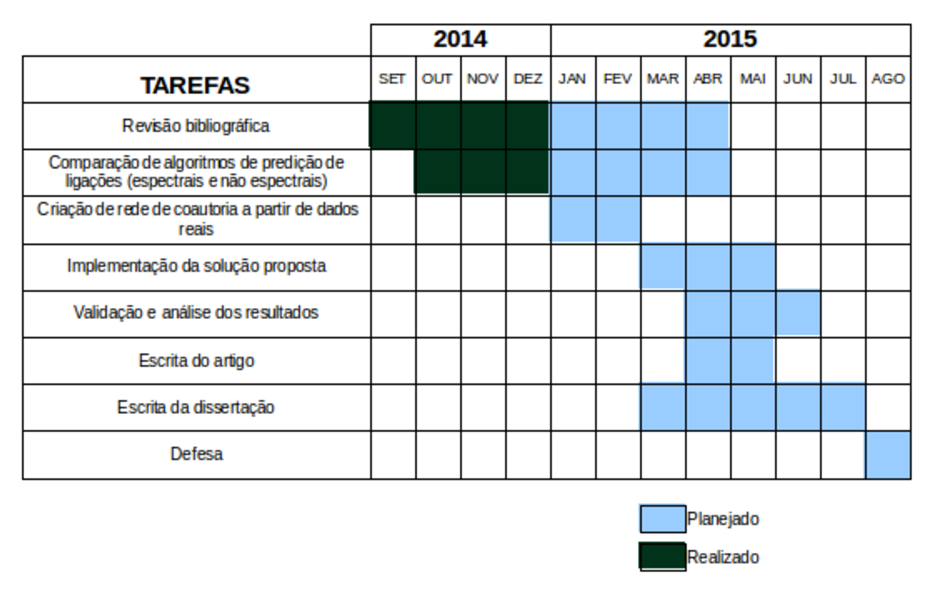
\includegraphics[width=0.9\textwidth]{cronograma.eps}
	\caption{Cronograma da Proposta de Disserta\c{c}\~{a}o.}
	\label{fig:cronograma}
\end{figure}





% -----
% PARTE DE REFERÊCIAS BIBLIOGRÁFICAS DA DISSERTAÇÃO
%
%  As referências da Proposta de Dissertação devem estar no arquivo refs.bib
%  Devem seguir o formato bibtex - ver Manual-Referencias.pdf para mais detalhes.
% -----
\bibliographystyle{proposta}
\bibliography{refs}


% -----
% PARTE DE ASSINATURAS DE SUA PROPOSTA DE DISSERTAÇÃO
% -----
\preparatitulos
\makeassinaturas


% -----
% FIM DO DOCUMENTO DE SUA PROPOSTA DE DISSERTAÇÃO
% -----
\label{theend}
\end{document}
